% Preamble templated from Dhawal24112006/EE1030
\documentclass{beamer}
\mode<presentation>
\usepackage{amsmath}
\usepackage{amssymb}
%\usepackage{advdate}
\usepackage{adjustbox}
\usepackage{subcaption}
\usepackage{enumitem}
\usepackage{multicol}
\usepackage{mathtools}
\usepackage{listings}
\usepackage{url}
\def\UrlBreaks{\do\/\do-}
\usetheme{Boadilla}
\usecolortheme{lily}
\setbeamertemplate{footline}
{
  \leavevmode%
  \hbox{%
  \begin{beamercolorbox}[wd=\paperwidth,ht=2.25ex,dp=1ex,right]{author in head/foot}%
    \insertframenumber{} / \inserttotalframenumber\hspace*{2ex}
  \end{beamercolorbox}}%
  \vskip0pt%
}
\setbeamertemplate{navigation symbols}{}

\providecommand{\nCr}[2]{\,^{#1}C_{#2}} % nCr
\providecommand{\nPr}[2]{\,^{#1}P_{#2}} % nPr
\providecommand{\mbf}{\mathbf}
\providecommand{\pr}[1]{\ensuremath{\Pr\left(#1\right)}}
\providecommand{\qfunc}[1]{\ensuremath{Q\left(#1\right)}}
\providecommand{\sbrak}[1]{\ensuremath{{}\left[#1\right]}}
\providecommand{\lsbrak}[1]{\ensuremath{{}\left[#1\right.}}
\providecommand{\rsbrak}[1]{\ensuremath{{}\left.#1\right]}}
\providecommand{\brak}[1]{\ensuremath{\left(#1\right)}}
\providecommand{\lbrak}[1]{\ensuremath{\left(#1\right.}}
\providecommand{\rbrak}[1]{\ensuremath{\left.#1\right)}}
\providecommand{\cbrak}[1]{\ensuremath{\left\{#1\right\}}}
\providecommand{\lcbrak}[1]{\ensuremath{\left\{#1\right.}}
\providecommand{\rcbrak}[1]{\ensuremath{\left.#1\right\}}}
\theoremstyle{remark}
\newtheorem{rem}{Remark}
\newcommand{\sgn}{\mathop{\mathrm{sgn}}}
\providecommand{\abs}[1]{\left\vert#1\right\vert}
\providecommand{\res}[1]{\Res\displaylimits_{#1}}
\providecommand{\norm}[1]{\lVert#1\rVert}
\providecommand{\mtx}[1]{\mathbf{#1}}
\providecommand{\mean}[1]{E\left[ #1 \right]}
\providecommand{\fourier}{\overset{\mathcal{F}}{ \rightleftharpoons}}
%\providecommand{\hilbert}{\overset{\mathcal{H}}{ \rightleftharpoons}}
\providecommand{\system}{\overset{\mathcal{H}}{ \longleftrightarrow}}
	%\newcommand{\solution}[2]{\textbf{Solution:}{#1}}
%\newcommand{\solution}{\noindent \textbf{Solution: }}
\providecommand{\dec}[2]{\ensuremath{\overset{#1}{\underset{#2}{\gtrless}}}}
\newcommand{\myvec}[1]{\ensuremath{\begin{pmatrix}#1\end{pmatrix}}}
\let\vec\mathbf

\lstset{
%language=C,
frame=single,
breaklines=true,
columns=fullflexible,
showstringspaces=false
}

\numberwithin{equation}{section}

\title{MATGEO Presentation: 1.10.18}
\author{Subhodeep Chakraborty \\ ee25btech11055,\\IIT Hyderabad.}

\date{\today}
\begin{document}

\begin{frame}
\titlepage
\end{frame}

\section*{Outline}
\begin{frame}
\tableofcontents
\end{frame}

\section{Problem}
\begin{frame}
\frametitle{Problem Statement}

Write the direction ratios of the vector $\vec{a} = \hat{\imath} + \hat{\jmath} - \hat{k}$ and hence calculate its direction cosines.

\end{frame}

\section{Solution}
\subsection{Direction Ratios}
\begin{frame}{Direction Ratios}
Given vector:
\begin{align}
 \vec{a} &= \myvec{1 \\ 1 \\ -1}
\end{align}
$\therefore$ The direction ratios are 1, 1 and -1.
\end{frame}

\subsection{Direction Cosines}
\begin{frame}{Direction Cosines}
Now,
\begin{align*}
\norm{\vec{a}} = \sqrt{3} \\
\implies \frac{\vec{a}}{\norm{\vec{a}}} = \myvec{\frac{1}{\sqrt{3}} \\ \frac{1}{\sqrt{3}} \\ \frac{-1}{\sqrt{3}}}
\end{align*}
Thus we see that the direction cosines are $1/\sqrt{3}$, $1/\sqrt{3}$ and $-1/\sqrt{3}$.
\end{frame}

\subsection{Plot}
\begin{frame}{Plot}
 \begin{figure}[H]
    \centering
    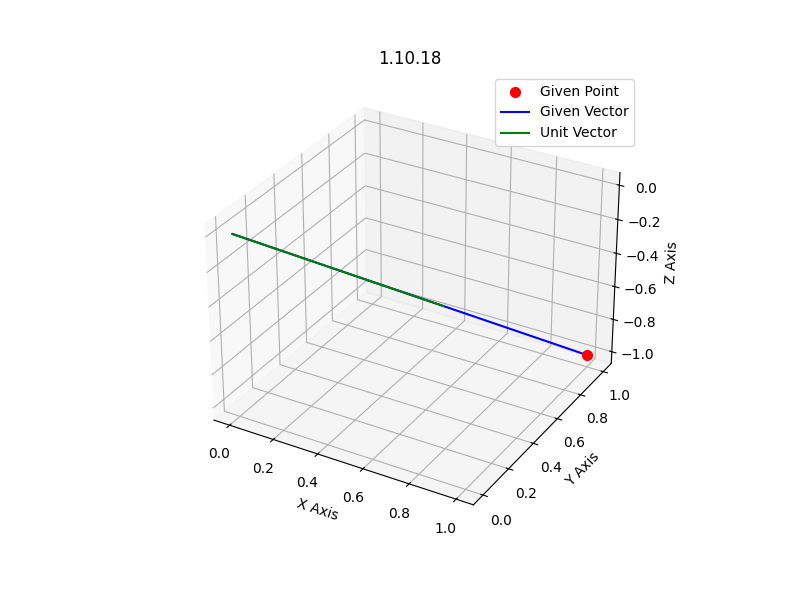
\includegraphics[width=\columnwidth]{../figs/plot.png}
    \caption*{}
    \label{fig:plot}
\end{figure}
\end{frame}
\section{C Code}
\begin{frame}[fragile]{C code for generating points on line}
\begin{lstlisting}[language=C]
void point_gen(const double* P1, const double* P2, double t, double* result_point) {
    result_point[0] = P1[0] + t * (P2[0] - P1[0]);
    result_point[1] = P1[1] + t * (P2[1] - P1[1]);
    result_point[2] = P1[2] + t * (P2[2] - P1[2]);
}
\end{lstlisting}
\end{frame}
\section{Python Code}
\subsection{Using C shared objects}
\begin{frame}[fragile]{Python code for plotting using C}
\begin{lstlisting}[language=Python]
import ctypes
import numpy as np
import matplotlib.pyplot as plt
from mpl_toolkits.mplot3d import Axes3D

lib = ctypes.CDLL("./line.so")

get_point = lib.point_gen
get_point.argtypes = [
    ctypes.POINTER(ctypes.c_double),  # P1
    ctypes.POINTER(ctypes.c_double),  # P2
    ctypes.c_double,  # t
    ctypes.POINTER(ctypes.c_double),  # result_point
]
get_point.restype = None
\end{lstlisting}
\end{frame}

\begin{frame}[fragile]{Python code for plotting using C}
\begin{lstlisting}[language=Python]
DoubleArray3 = ctypes.c_double * 3
P1_arr = DoubleArray3(0, 0, 0)
P2_arr = DoubleArray3(1, 1, -1)

t_values = np.linspace(0, 1, 100)
line_points_x, line_points_y, line_points_z = [], [], []

for t in t_values:
    result_arr = DoubleArray3()

    get_point(P1_arr, P2_arr, t, result_arr)

    line_points_x.append(result_arr[0])
    line_points_y.append(result_arr[1])
    line_points_z.append(result_arr[2])

point = np.array([1, 1, -1])

\end{lstlisting}
\end{frame}

\begin{frame}[fragile]{Python code for plotting using C}
\begin{lstlisting}[language=Python]
fig = plt.figure(figsize=(8, 6))
ax = fig.add_subplot(111, projection="3d")
x, y, z = point
ax.scatter(
    x,
    y,
    z,
    color="red",
    s=50,
    label="Given Point",
)

\end{lstlisting}
\end{frame}

\begin{frame}[fragile]{Python code for plotting using C}
\begin{lstlisting}[language=Python]
ax.plot(
    line_points_x,
    line_points_y,
    line_points_z,
    color="blue",
    label="Given Vector",
)

unit_vec = point / LA.norm(point)
unit = list(unit_vec)
x, y, z = unit
P3_arr = DoubleArray3(x, y, z)
t_values = np.linspace(0, 1, 100)
line_points_x, line_points_y, line_points_z = [], [], []

\end{lstlisting}
\end{frame}

\begin{frame}[fragile]{Python code for plotting using C}
\begin{lstlisting}[language=Python]
for t in t_values:
    result_arr = DoubleArray3()

    get_point(P1_arr, P3_arr, t, result_arr)

    line_points_x.append(result_arr[0])
    line_points_y.append(result_arr[1])
    line_points_z.append(result_arr[2])

ax.plot(
    line_points_x,
    line_points_y,
    line_points_z,
    color="green",
    label="Unit Vector",
)
\end{lstlisting}
\end{frame}

\begin{frame}[fragile]{Python code for plotting using C}
 \begin{lstlisting}[language=Python]
  ax.set_xlabel("X Axis")
ax.set_ylabel("Y Axis")
ax.set_zlabel("Z Axis")
ax.set_title("1.10.18")
ax.legend()
ax.grid(True)

plt.savefig("../figs/plot.png")
plt.show()
 \end{lstlisting}
\end{frame}

\subsection{Plot}
\begin{frame}{Plot}
 \begin{figure}[H]
    \centering
    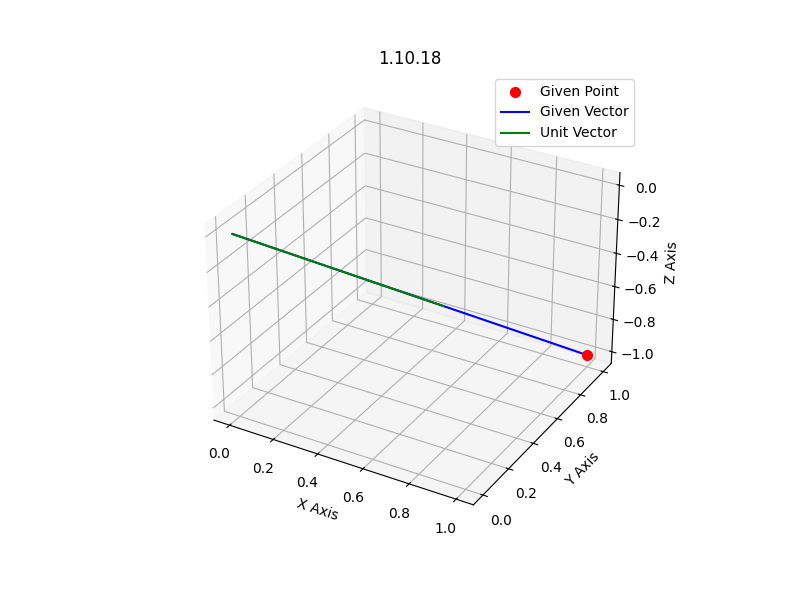
\includegraphics[width=\columnwidth]{../figs/plot.png}
    \caption*{}
    \label{fig:plot_c}
\end{figure}
\end{frame}

\subsection{In Pure Python}
\begin{frame}[fragile]{Pure Python Code for Plotting}
\begin{lstlisting}[language=Python]
import numpy as np
import numpy.linalg as LA
import matplotlib.pyplot as plt
from mpl_toolkits.mplot3d import Axes3D

vec = np.array([1, 1, -1]).reshape(-1, 1)

# Solving
print(f"Direction ratios are {vec[0]}, {vec[1]}, {vec[2]}")
unit = vec / LA.norm(vec)
print(f"Direction cosines are {unit[0]}, {unit[1]}, {unit[2]}")

\end{lstlisting}
\end{frame}

\begin{frame}[fragile]{Pure Python Code for Plotting}
\begin{lstlisting}[language=Python]
# Plotting

fig = plt.figure(figsize=(8, 8))
ax = fig.add_subplot(111, projection="3d")

x, y, z = vec
ax.scatter(x, y, z, color="red", s=50, label="Given Point")
ax.quiver(
    0, 0, 0, x, y, z, color="blue", arrow_length_ratio=0.1, label="Position Vector"
)
x, y, z = unit
ax.quiver(0, 0, 0, x, y, z, color="green", arrow_length_ratio=0.1, label="Unit Vector")
\end{lstlisting}
\end{frame}

\begin{frame}[fragile]{Pure Python Code for Plotting}
\begin{lstlisting}[language=Python]
 ax.set_xlabel("X-axis")
ax.set_ylabel("Y-axis")
ax.set_zlabel("Z-axis")
ax.set_title("1.10.18")
ax.legend()
ax.grid(True)

plt.savefig("../figs/python.png")
plt.show()
\end{lstlisting}
\end{frame}

\subsection{Plot}
\begin{frame}{Pure Python Plot}
 \begin{figure}[H]
    \centering
    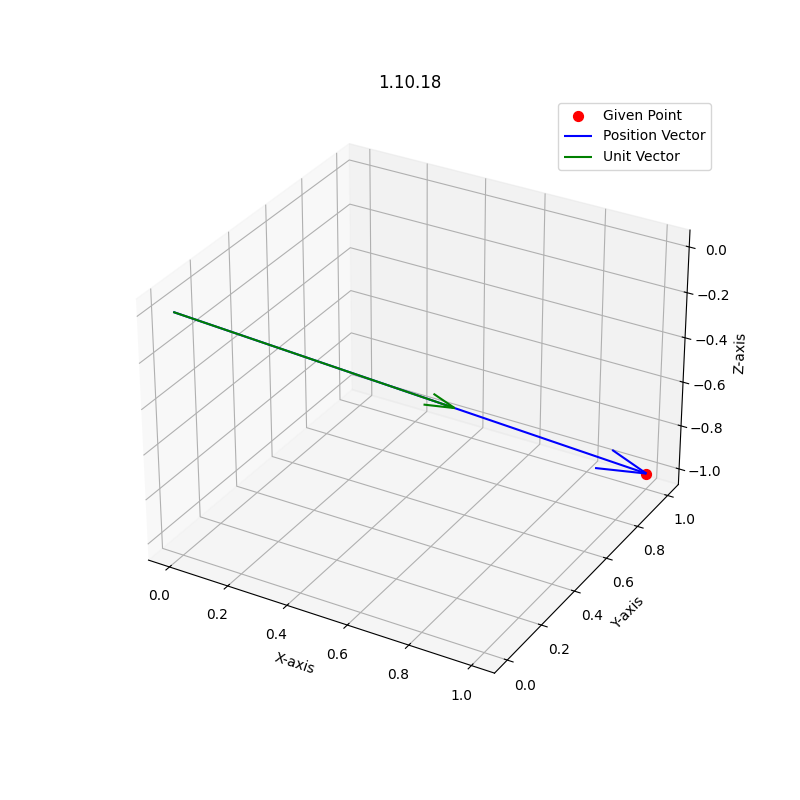
\includegraphics[width=0.75\columnwidth]{../figs/python.png}
    \caption*{}
    \label{fig:plot_p}
\end{figure}
\end{frame}
\end{document}
